\documentclass[12pt,a4paper,oneside, reqno]{amsart}
\usepackage{changepage}
\usepackage{mathtext} % русские буквы в формулах
\usepackage[T2A]{fontenc}
\usepackage[utf8x]{inputenc}
\usepackage{ucs}
\usepackage{cmap}
\usepackage[english,russian]{babel}
\usepackage{graphicx}
\usepackage{concrete}
\usepackage{amsmath}
\usepackage{amsfonts}
\usepackage{amssymb}
\usepackage{dcolumn}
\usepackage{booktabs}
\usepackage{ctable}
\usepackage{multirow}
\usepackage{float}
\restylefloat{table}

\newcommand{\specialcell}[2][c]{%
  \begin{tabular}[#1]{@{}c@{}}#2\end{tabular}}
\oddsidemargin = 0pt
\textwidth = 14 cm
\topmargin = -2 cm
\textheight = 24 cm
\makeatletter
\renewcommand{\theequation}{\thesection.\arabic{equation}}
\@addtoreset{equation}{section}
\newcommand{\eq}{\begin{equation}}
\newcommand{\eeq}{\end{equation}}
\newcommand{\fr}{\frac}
\newcommand{\mf}{\mathfrak}
\newcommand{\sub}{\subsection}
\newcommand{\subsub}{\subsubsection}
\newcommand{\definition}{\theoremstyle{definition}}
\newcommand{\mult}[2]{\genfrac{\left[}{\right.}{0pt}{}{#1}{#2}}
\renewcommand{\qed}{\begin{center} $\mathsf{QED}$ \end{center}}
\newcommand{\al}{\alpha}
\newcommand{\comment}[1]{\marginpar{\Small{{\sl #1}}} }
\newcommand{\epigraph}[2]{\begin{flushright} {\em #1}\\#2\\[20 pt]
\end{flushright}}
\newcommand{\fx}[1]{\ensuremath{\mathit{f}_{#1}(x)}}
\newcommand{\re}[1]{(\ref{#1})}
\newcommand{\mh}{\mathit}
\newcommand{\itm}[1]{\begin{itemize}	\item #1 \end{itemize}}
\newcommand{\note}[1]{\begin{flushleft}\hbox{%
\vrule\hspace{.5em}\parbox{ .9\textwidth}%
{ #1}} \end{flushleft}}
\newcommand{\Al}{\ensuremath{\mathcal{A}}}
\newcommand{\@dotsep}{3.9}
\newcommand{\system}[1]{\eq\left\{ \begin{aligned} #1
\end{aligned}\right.\\[5 pt]\eeq}
\renewcommand{\phi}{\varphi}

% http://www.texnik.de/floats/caption.phtml
% This does spacing around caption.
%\setlength{\abovecaptionskip}{6pt}   % 0.5cm as an example
%\setlength{\belowcaptionskip}{9pt}   % 0.5cm as an example

%%%%%%%%%%%%%%%%%%%%%%%%%%%%%%%%%%%%%%%%%%%%%%%%%%%%%%%%%%%%%%%%%%%%%%%

\begin{document}
\tableofcontents
\newpage
\section{Цель Работы}
\begin{itemize}
    \item Изучить основные понятия, характеризующие явление дифракции.\\
    \item Изучить метод строгого решения дифракционной задачи на бесконечном идеально проводящем цилиндре.\\
    \item Изучить метод приближенного решения дифракционной задачи --- метод волновой оптики --- на примере
          отверстия в плоском проводящем экране бесконечных размеров.\\
    \item Изучить метод приближенного решения дифракционной задачи --- метод геометрической оптики --- на 
          примере бесконечного идеально проводящего цилиндра.\\
    \item Построить математическую модель процесса дифракции плоской волны на цилиндре и отверстии в экране
          и разработать программу расчёта дифрагированных полей.\\
    \item Изучить методы измерения дифрагированных полей.\\
    \item Исследовать явления дифракции электромагнитных волн на цилиндре и отверстии.
\end{itemize}

\newpage
\section{Таблицы результатов измерений и вычислений}
{\small
\begin{table}[H]
\newcolumntype{W}{D{.}{.}{2.3}}
\begin{adjustwidth}{-1.5cm}{}
\vspace{10pt}
\begin{tabular}{ccWWWWWWWWW} \toprule %[-2.08em]
\newcolumntype{W}{D{.}{.}{2.3}}
%\specialcell{Gain\\threshold, \%}	&	\specialcell{JLSv2,\\number of files}	&	\specialcell{JPEG-2k,\\number of files}\\
\multirow{2}*{$\theta^\circ$} & \multirow{2}*{\specialcell{Поле без пре-\\пятствий, $l_0$}} & \multicolumn{3}{c}{$d=8$mm} & \multicolumn{3}{c}{$d=16$mm} & \multicolumn{3}{c}{$d=32$mm}\\
& & \multicolumn{1}{c}{$l_1$} & \multicolumn{1}{c}{$\Delta_1=l_0-l_1$} &
\multicolumn{1}{c}{$\Delta_{1n}$} & 
\multicolumn{1}{c}{$l_2$} & \multicolumn{1}{c}{$\Delta_2=l_0-l_2$} & 
\multicolumn{1}{c}{$\Delta_{2n}$} & 
\multicolumn{1}{c}{$l_3$} & \multicolumn{1}{c}{$\Delta_3=l_0-l_3$} & 
\multicolumn{1}{c}{$\Delta_{3n}$}\\
 \midrule
0.00 & 37.0 & 22.0 & 15.0 & 0.65 & 22.0 & 15.0 & 0.56 & 15.0 & 22.0 & 0.56\\
5.00 & 52.0 & 33.0 & 19.0 & 0.83 & 29.0 & 23.0 & 0.85 & 17.0 & 35.0 & 0.9\\
10.0 & 56.0 & 33.0 & 23.0 & 1.0 & 31.0 & 25.0 & 0.93 & 17.0 & 39.0 & 1.0\\
15.0 & 44.0 & 32.0 & 12.0 & 0.52 & 22.0 & 22.0 & 0.81 & 12.0 & 32.0 & 0.82\\
20.0 & 43.0 & 36.0 & 7.0 & 0.3 & 31.0 & 12.0 & 0.44 & 34.0 & 9.0 & 0.23\\
25.0 & 43.0 & 57.0 & -14.0 & -0.6 & 58.0 & -15.0 & -0.55 & 60.0 & -17.0 & -0.43\\
30.0 & 35.0 & 49.0 & -14.0 & -0.6 & 50.0 & -15.0 & -0.55 & 65.0 & -30.0 & -0.77\\
35.0 & 24.0 & 29.0 & -5.0 & -0.22 & 33.0 & -9.0 & -0.33 & 50.0 & -26.0 & -0.66\\
40.0 & 50.0 & 33.0 & 17.0 & 0.74 & 23.0 & 27.0 & 1.0 & 17.0 & 33.0 & 0.85\\
45.0 & 60.0 & 57.0 & 3.0 & 0.13 & 49.0 & 11.0 & 0.4 & 42.0 & 18.0 & 0.46\\
\bottomrule
\end{tabular}
\caption{Дифракция ЭМВ на цилиндре.} 
\end{adjustwidth}
\label{tab:table3}
\end{table}
}
% We need 4 more tables here!
\begin{table}[hb]
\centering
\vspace{-10pt}
\begin{tabular}{cccc} \toprule %[-2.08em]
    \text{Диаметр цилиндра} & $l(100)$ & $l(150)$ & $l(200)$ \\
\midrule
0 & 50 & 36 & 22\\
8 & 30 & 22 & 13\\
16 & 21 & 14 & 12\\
32 & 12 & 10 & 9\\
\bottomrule
\end{tabular}
\caption{Величина напряженности электрического поля, дифрагированного в 
область геометрической тени цилиндра.} 
\label{tab:table1}
\end{table}

\begin{table}[hb]
\centering
\begin{tabular}{cccc} \toprule %[-2.08em]
$\theta^\circ$ & $\alpha=32$mm & $\alpha=64$mm & $\alpha=100$mm \\
\midrule
0 & 4 & 23 & 24\\
5 & 5 & 25 & 21\\
10 & 6 & 28 & 15\\
15 & 6 & 29 & 6\\
20 & 7 & 14 & 3\\
25 & 9 & 11 & 3\\
30 & 6 & 4 & 3\\
35 & 5 & 2 & 4\\
40 & 3 & 1 & 2\\
45 & 2 & 1 & 1\\
\bottomrule
\end{tabular}
\caption{Дифракция ЭМВ на щели.} 
\label{tab:table2}
\end{table}
\newpage

\section{Графики и рисунки}
\begin{figure}[h!b]
    \centering
    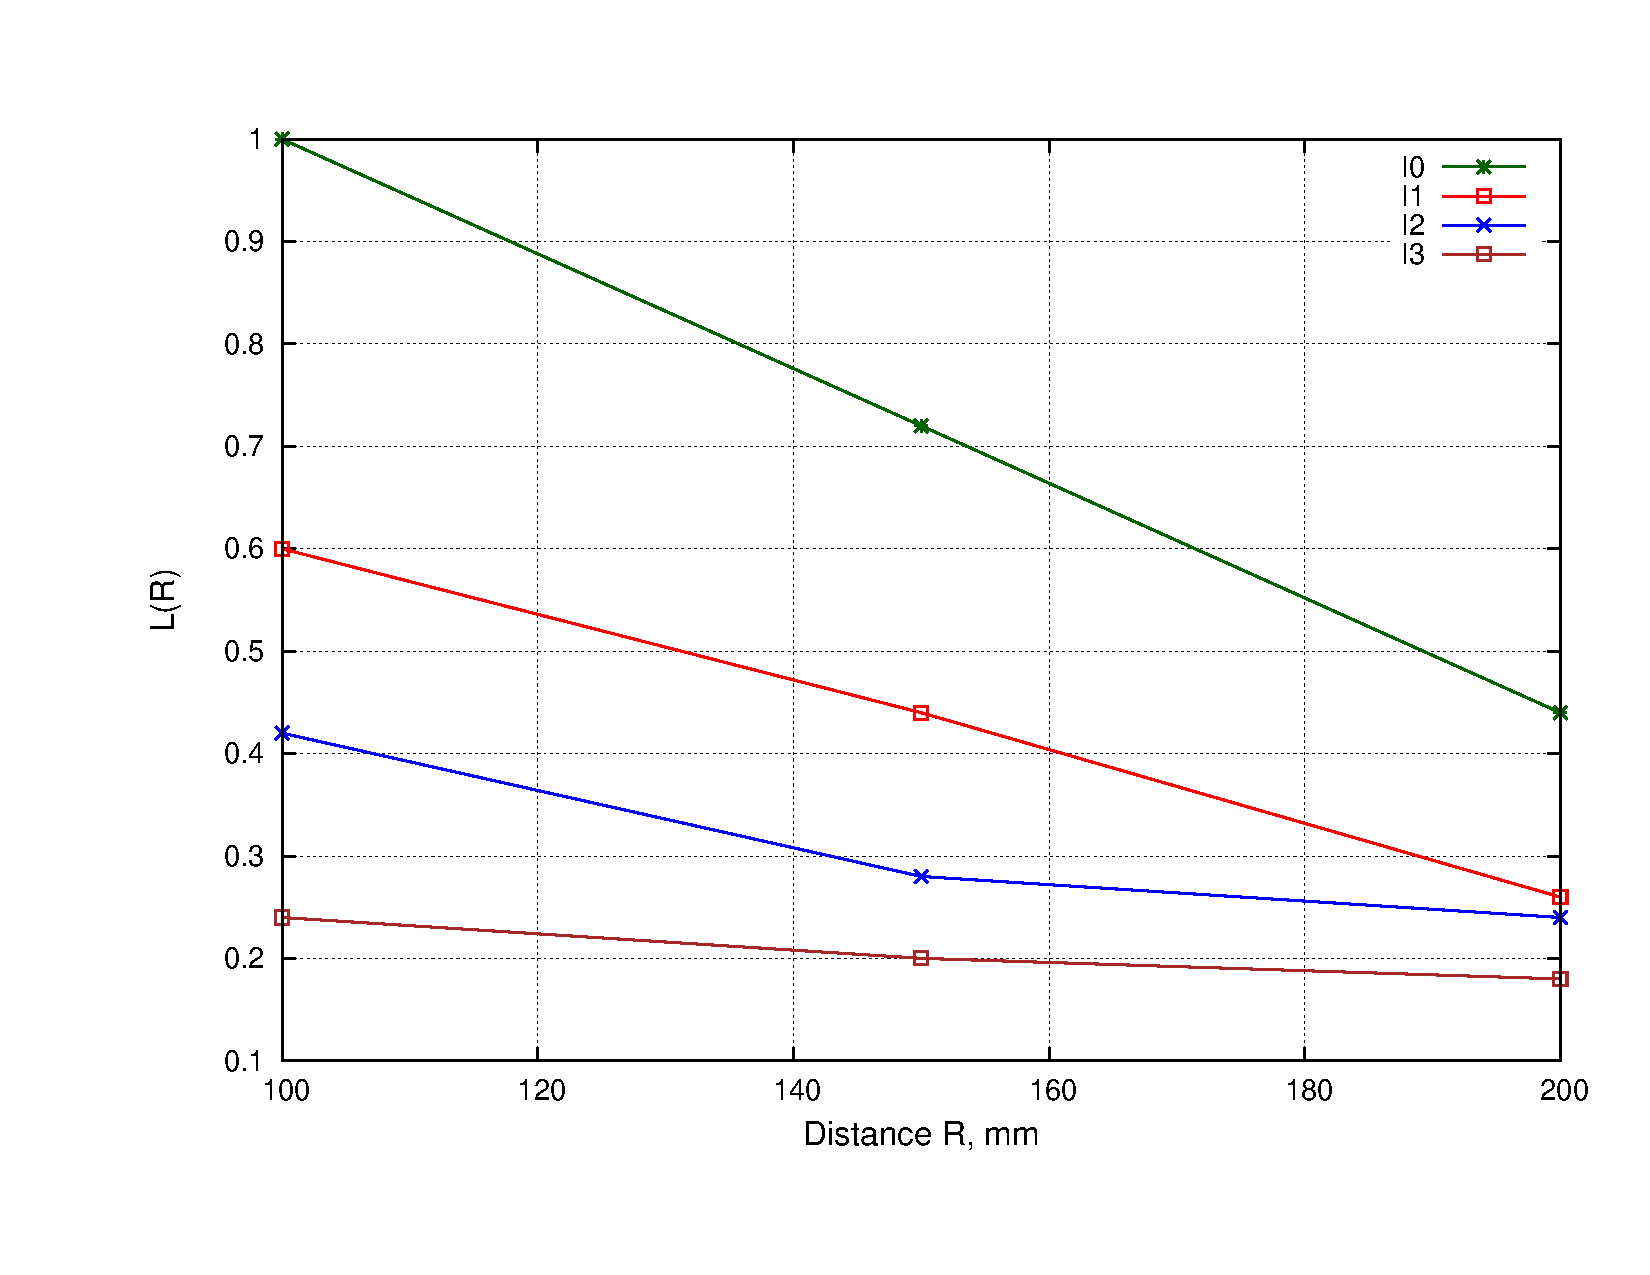
\includegraphics[width = \textwidth]{plot1.pdf}
    \vspace{-30pt}
    \caption{График зависимости величины ЭМП в области геометрической тени от расстояния до цилиндра.}
    \label{fig:plot1}
\end{figure}

\begin{figure}
    \centering
    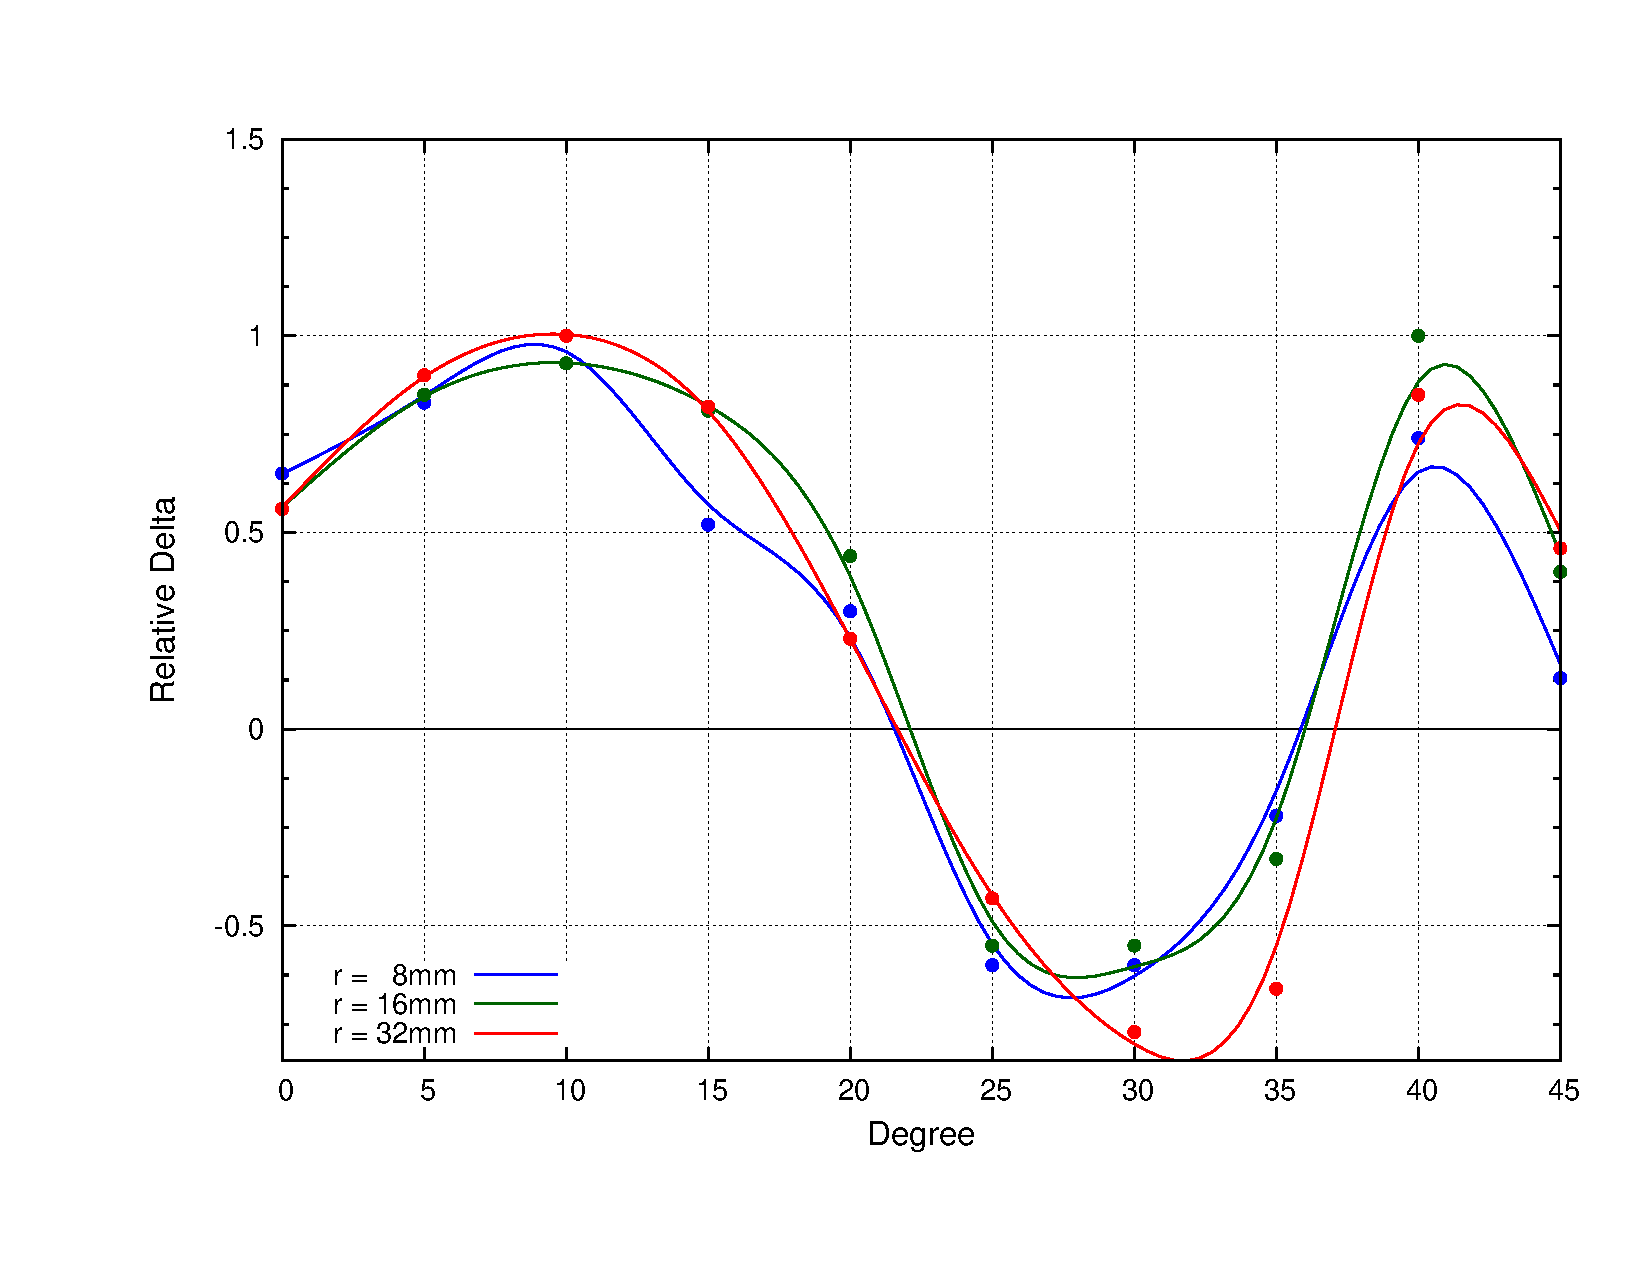
\includegraphics[width = \textwidth]{plot2.pdf}
    \vspace{-30pt}
    \caption{График зависимости величины ЭМП от угла преломления ЭМВ на цилиндре.}
    \label{fig:plot2}
\end{figure}

\begin{figure}
    \centering
    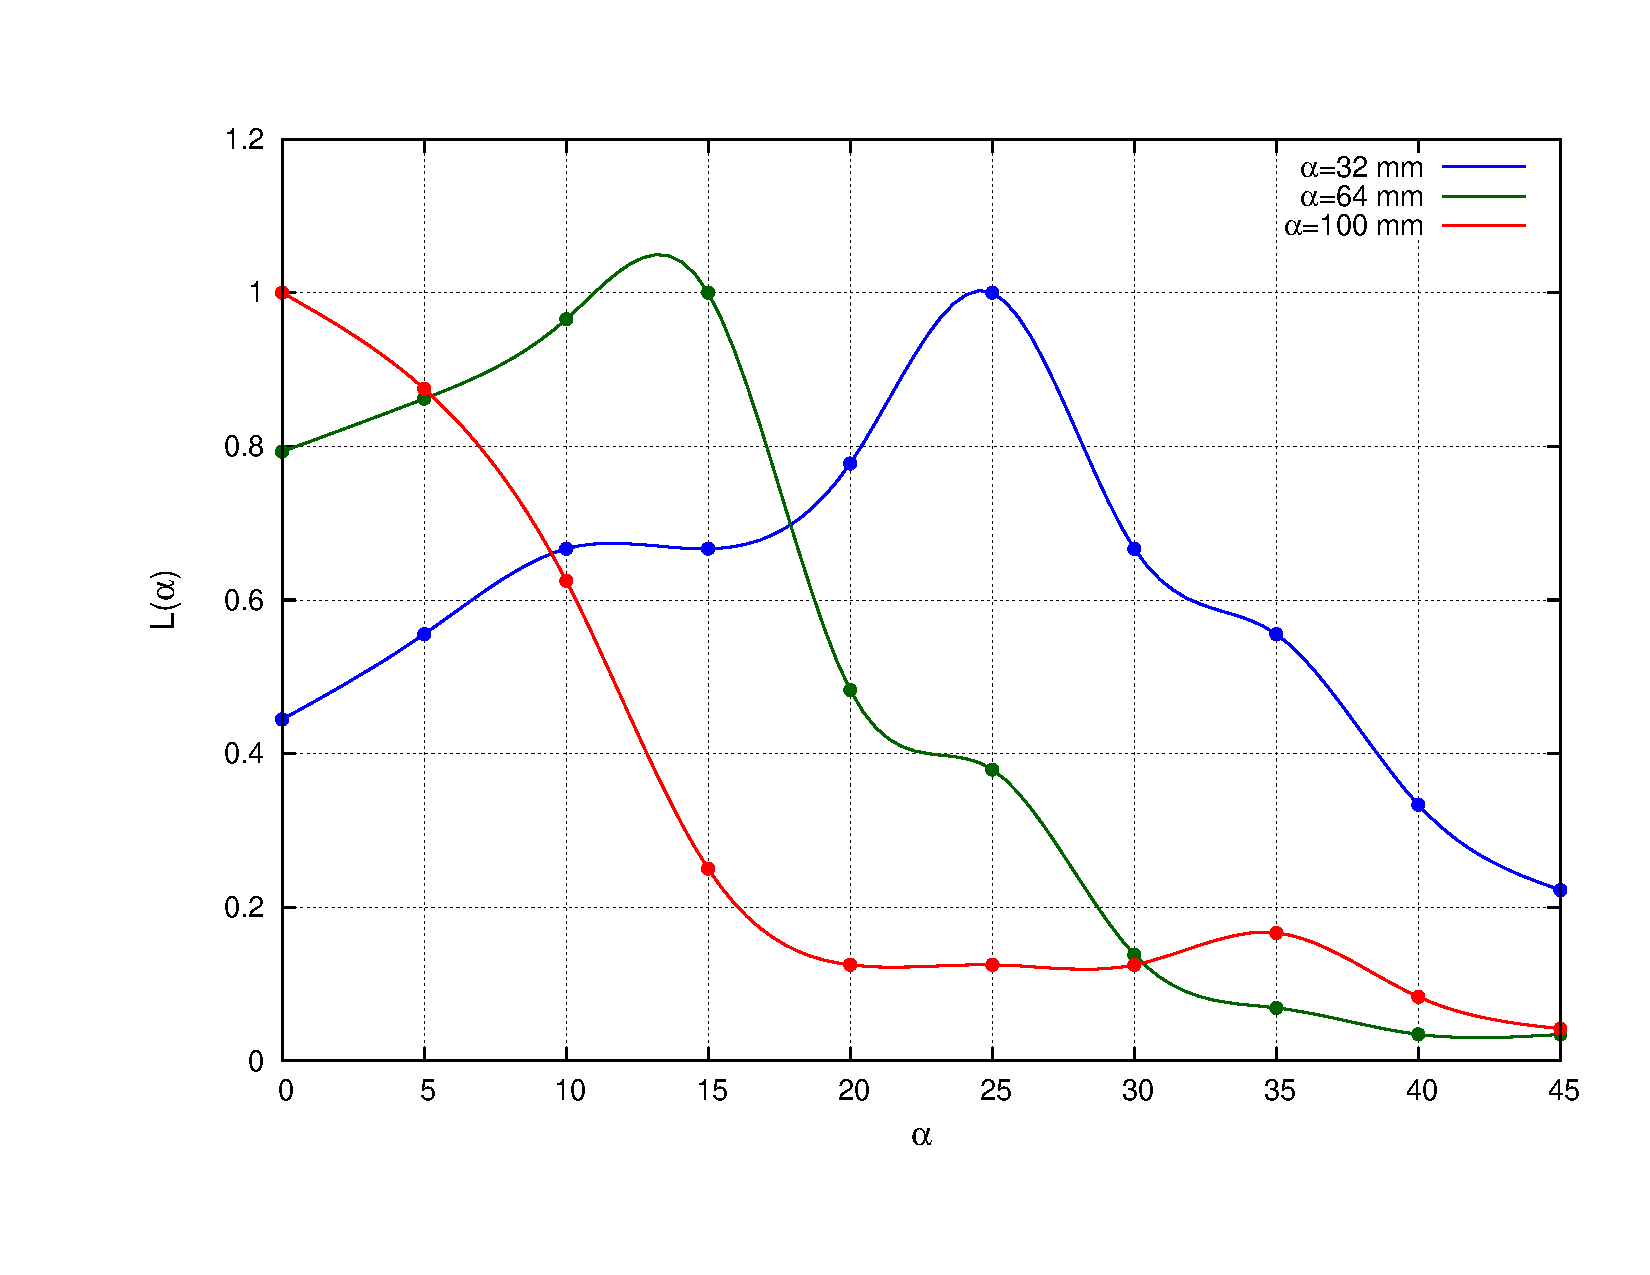
\includegraphics[width = \textwidth]{plot3.pdf}
    \vspace{-30pt}
    \caption{График зависимости величины ЭМП от угла преломления ЭМВ на щели.}
    \label{fig:plot3}
\end{figure}

\begin{figure}
    \centering
    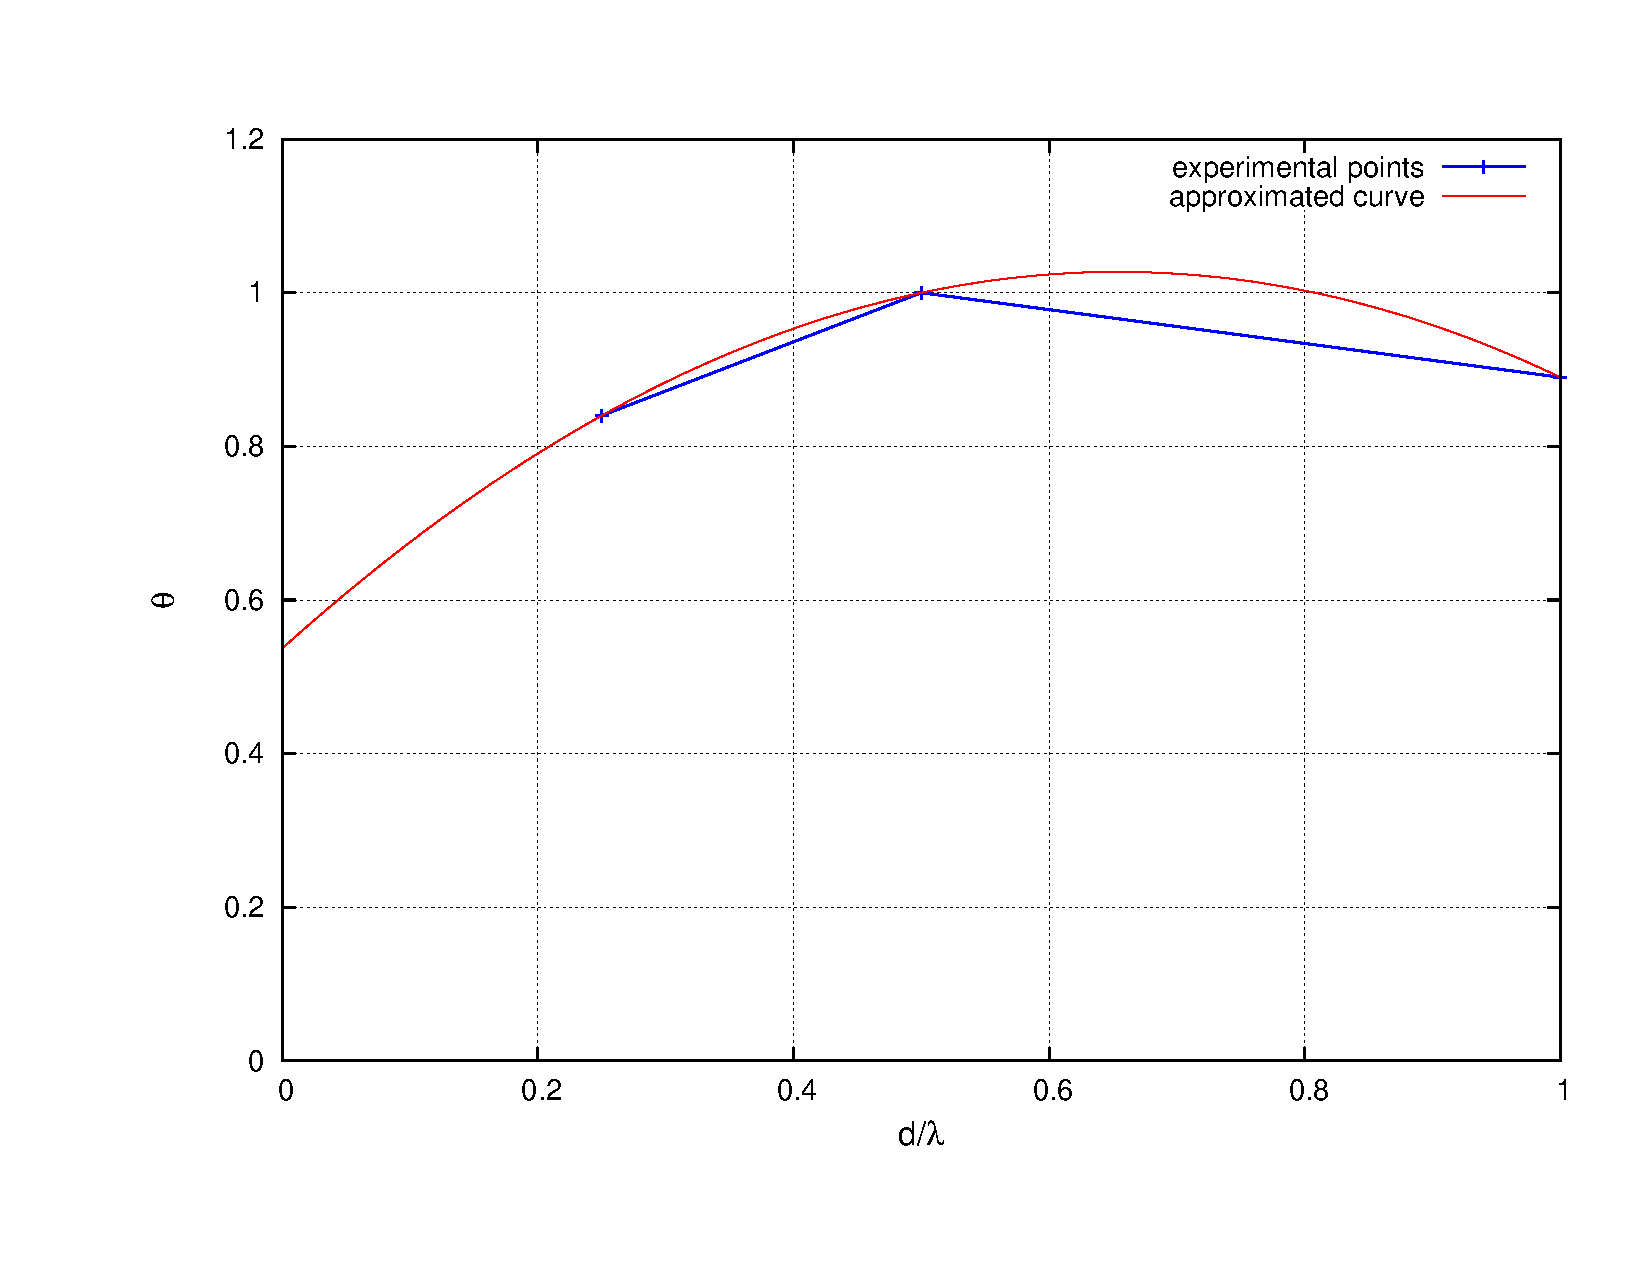
\includegraphics[width = \textwidth]{plot4-1.pdf}
    \vspace{-30pt}
    \caption{График зависимости угла половинной мощности от нормированных размеров цилиндра.}
    \label{fig:plot4}
\end{figure}

\begin{figure}
    \centering
    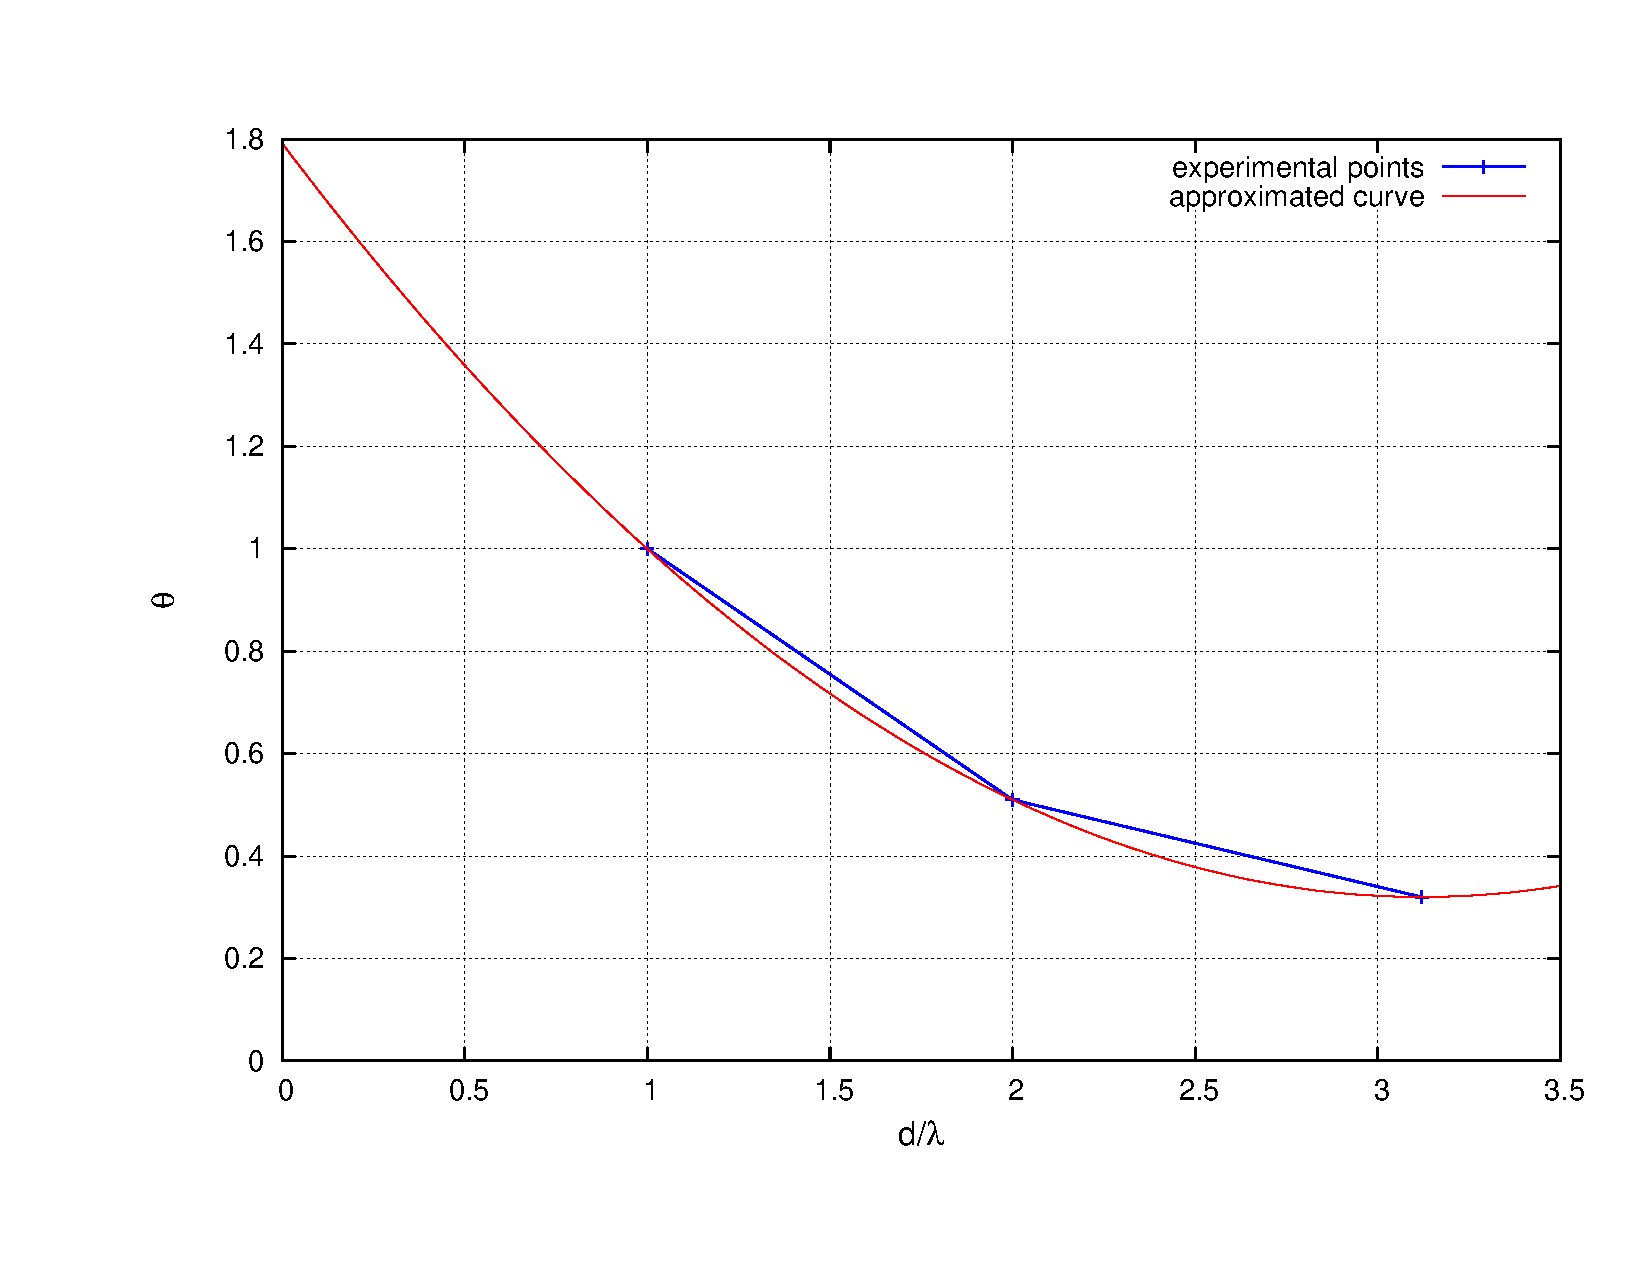
\includegraphics[width = \textwidth]{plot4-2.pdf}
    \vspace{-30pt}
    \caption{График зависимости угла половинной мощности от нормированных размеров щели.}
    \label{fig:plot5}
\end{figure}

\newpage
\section{Выводы}
Как видно из рис. 1, энергия волны падает по мере удаления от иссточника. Величина энергии прямо пропорциональна размерам препятствия, а скорость убывания - обратно пропорциональна. Рис. 2 показывает кривую зависимости мощности волны от угла отклонения приемника. Наличие ярко выраженных пиков на кривой подтверждает факт наличия явления интерференции. На рис. 3 наблюдается то же явление, однако отличие в интерференции на щели характеризуется сдвигом пика кривой по оси угла отклонения приемника. Этот факт объясняется значительным смещением точек дифракции в зависимости от ширины щели. На основании этих данных построены графики на рис. 4 и рис. 5, на которых отражена экспериментальная и построенная на экспериментальных данных теоретическая кривые зависимости нормированного угла половинной мощности волны к размеру препятствия (рис. 4) и щели (рис. 5) относительно длины волны. 
\end{document}
